\section{Результаты тестирования}
\label{sec:tests}

Визуальное сравнение исходных и восстановленных изображений приведено на рисунках~\ref{fig:cmp-smooth}--\ref{fig:cmp-texture}. Все изображения восстановлены в исходном разрешении $256 \times 256$; перекрывающиеся блоки при сборке усреднялись.

\begin{figure}[H]
	\centering
	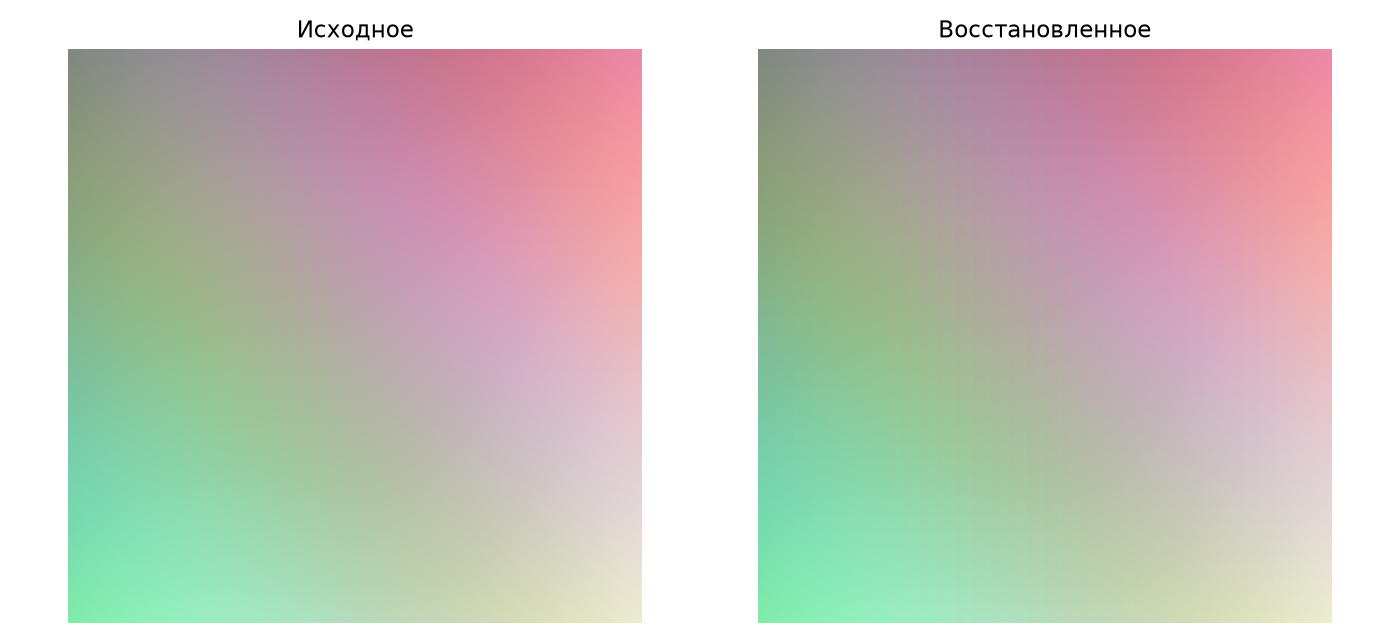
\includegraphics[width=0.95\textwidth]{compare_smooth.png}
	\caption{Плавные переходы: исходное и восстановленное изображения}
	\label{fig:cmp-smooth}
\end{figure}

\begin{figure}[H]
	\centering
	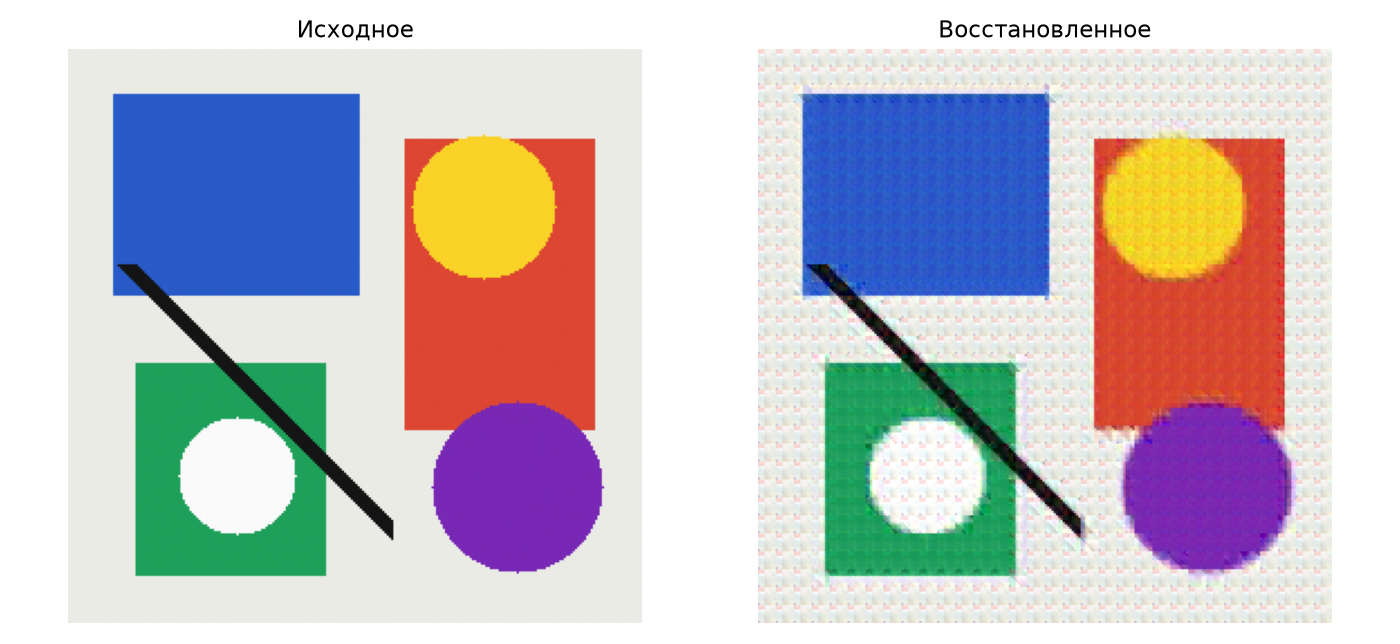
\includegraphics[width=0.95\textwidth]{compare_contours.png}
	\caption{Контуры: исходное и восстановленное изображения}
	\label{fig:cmp-contours}
\end{figure}

\begin{figure}[H]
	\centering
	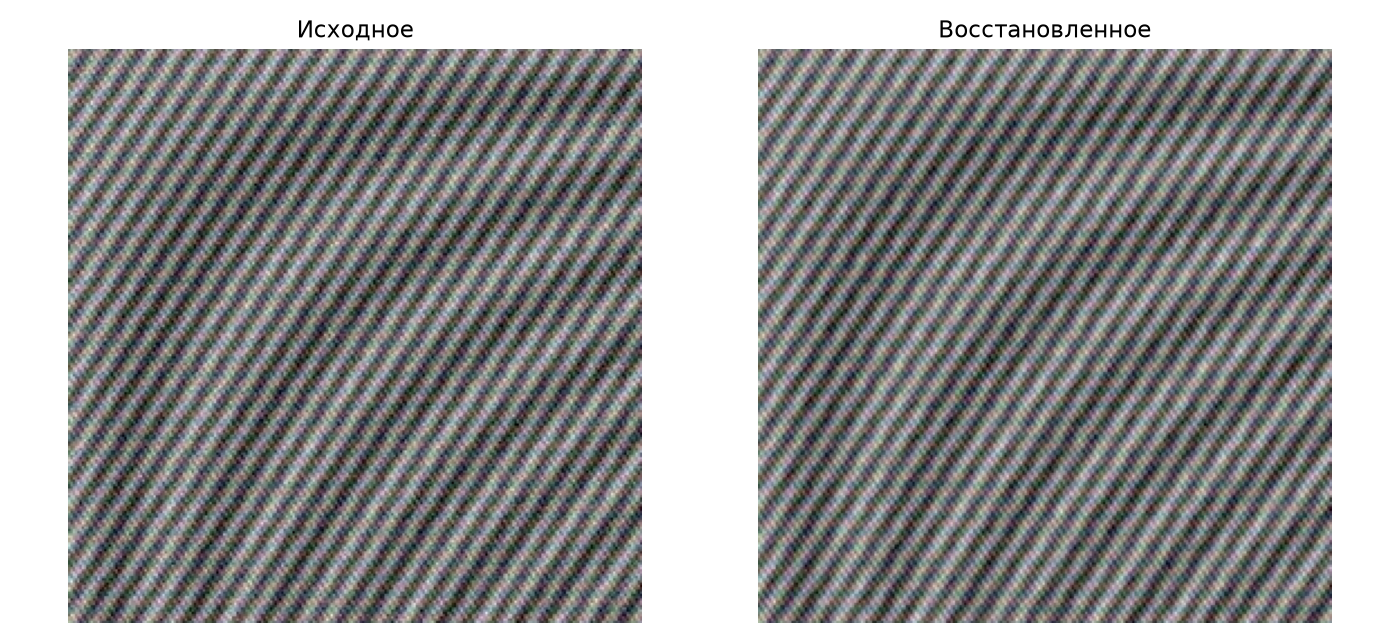
\includegraphics[width=0.95\textwidth]{compare_texture.png}
	\caption{Текстура: исходное и восстановленное изображения}
	\label{fig:cmp-texture}
\end{figure}

Для плавных переходов восстановление визуально почти неотличимо от оригинала: низкочастотный сигнал хорошо аппроксимируется линейным подпространством размерности $p=16$. На изображении с контурами сохраняются крупные области и общая геометрия, но границы становятся менее резкими. Для текстуры теряется часть мелких деталей, что согласуется с наибольшей остаточной ошибкой в таблице~\ref{tab:results}.

Ошибка готового BMP в шкале $0\ldots255$ и PSNR приведены в таблице~\ref{tab:results}. Эти значения отличаются от $\mathrm{MSE}_n$: перед сохранением выполняется ограничение диапазона, сборка с усреднением перекрытий и округление до \texttt{uint8}. Поэтому метрики нормированных блоков и готового изображения не смешиваются.

\subsection{Влияние перекрытия блоков}

Сравнение шагов $s_h=s_w=8$ (без перекрытия) и $s_h=s_w=4$ (перекрытие 50\%) приведено в таблице~\ref{tab:overlap}. При уменьшении шага число блоков $Q$ возрастает примерно в четыре раза (с 1024 до 3969). Поэтому байтовый коэффициент $K$ не улучшается, а ухудшается: он возрастает с 1{,}263 до 1{,}431, т.е. байтовое сжатие становится менее выгодным. Время обучения при этом также растёт пропорционально числу блоков.

Влияние усреднения на ошибку неоднозначно. Ошибка готового изображения уменьшается: PSNR возрастает для всех трёх изображений (для плавных переходов с 51{,}64 до 57{,}92~дБ, для контуров с 25{,}94 до 27{,}17~дБ, для текстуры с 26{,}16 до 27{,}33~дБ). Однако $\mathrm{MSE}_n$ нормированных блоков для контуров и текстуры немного возрастает (с 0{,}010536 до 0{,}011086 и с 0{,}009688 до 0{,}010012 соответственно), а для плавных переходов снижается с 0{,}000027 до 0{,}000010. Причина в том, что при перекрытии каждый блок восстанавливается по своей окрестности и усреднение сглаживает межблочные швы, но остаточная ошибка отдельного блока может слегка увеличиться.

\begin{table}[H]
\centering
\caption{Влияние перекрытия блоков ($p=16$)}
\label{tab:overlap}
\begin{tabular}{@{}lcccccc@{}}
\hline
Изображение & $s_h=s_w$ & $Q$ & $K$ & $T$ & $\mathrm{MSE}_n$ & PSNR, дБ \\
\hline
Плавные переходы & 8 & 1024 & 1{,}263 & 80 & 0{,}000027 & 51{,}64 \\
Плавные переходы & 4 & 3969 & 1{,}431 & 80 & 0{,}00001 & 57{,}92 \\
\hline
Контуры & 8 & 1024 & 1{,}263 & 80 & 0{,}010536 & 25{,}94 \\
Контуры & 4 & 3969 & 1{,}431 & 80 & 0{,}011086 & 27{,}17 \\
\hline
Текстура & 8 & 1024 & 1{,}263 & 80 & 0{,}009688 & 26{,}16 \\
Текстура & 4 & 3969 & 1{,}431 & 80 & 0{,}010012 & 27{,}33 \\
\hline
\end{tabular}
\end{table}


Таким образом, перекрытие является компромиссом: оно повышает визуальное качество и PSNR готового изображения за счёт сглаживания границ блоков, но требует хранить почти в четыре раза больше кодов и поэтому ухудшает байтовый коэффициент сжатия.
